\documentclass[12pt, titlepage]{article}

\usepackage[dvipsnames]{xcolor} % for different colour comments
\usepackage{tabto}
\usepackage{mdframed}
\mdfsetup{nobreak=true}
\usepackage{xkeyval}
\usepackage{tabularx}
\usepackage{booktabs}
\usepackage{hyperref}
\hypersetup{
    colorlinks,
    citecolor=black,
    filecolor=black,
    linkcolor=red,
    urlcolor=blue
}
\usepackage[skip=2pt, labelfont=bf]{caption}
\usepackage{titlesec}
\usepackage{placeins}
\usepackage{graphicx}
\graphicspath{ {image/} }



%% the following adds another section level by redefining the paragraph
%% source:  http://tex.stackexchange.com/questions/60209/how-to-add-an-extra-level-of-sections-with-headings-below-subsubsection
\setcounter{secnumdepth}{4}

\titleformat{\paragraph}
{\normalfont\normalsize\bfseries}{\theparagraph}{1em}{}
\titlespacing*{\paragraph}
{0pt}{3.25ex plus 1ex minus .2ex}{1.5ex plus .2ex}


%% Comments
\newif\ifcomments\commentstrue

\ifcomments
\newcommand{\authornote}[3]{\textcolor{#1}{[#3 ---#2]}}
\newcommand{\todo}[1]{\textcolor{red}{[TODO: #1]}}
\else
\newcommand{\authornote}[3]{}
\newcommand{\todo}[1]{}
\fi

\newcommand{\wss}[1]{\authornote{magenta}{SS}{#1}}
\newcommand{\ds}[1]{\authornote{blue}{DS}{#1}}



%% The following are used for pretty printing of events and requirements
\makeatletter

\define@cmdkey      [TP] {test}     {name}       {}
\define@cmdkey      [TP] {test}     {desc}       {}
\define@cmdkey      [TP] {test}     {type}       {}
\define@cmdkey      [TP] {test}     {init}       {}
\define@cmdkey      [TP] {test}     {input}      {}
\define@cmdkey      [TP] {test}     {output}     {}
\define@cmdkey      [TP] {test}     {pass}       {}
\define@cmdkey      [TP] {test}     {user}       {}
\define@cmdkey      [TP] {test}     {result}     {}


\newcommand{\getCurrentSectionNumber}{%
  \ifnum\c@section=0 %
  \thechapter
  \else
  \ifnum\c@subsection=0 %
  \thesection
  \else
  \ifnum\c@subsubsection=0 %
  \thesubsection
  \else
  \thesubsubsection
  \fi
  \fi
  \fi
}

\newcounter{TestNum}


\newcommand{\testauto}[1]{
\setkeys[TP]{test}{#1}
\refstepcounter{TestNum}
\begin{mdframed}[linewidth=1pt]
\begin{tabularx}{\textwidth}{@{}p{3cm}X@{}}
{\bf Test \#\theTestNum:} & {\bf \cmdTP@test@name}\\[\baselineskip]
{\bf Description:} & \cmdTP@test@desc\\[0.5\baselineskip]
{\bf Type:} & \cmdTP@test@type\\[0.5\baselineskip]
{\bf Initial State:} & \cmdTP@test@init\\[0.5\baselineskip]
{\bf Input:} & \cmdTP@test@input\\[0.5\baselineskip]
{\bf Output:} & \cmdTP@test@output\\[0.5\baselineskip]
{\bf Expected:} & \cmdTP@test@pass\\[\baselineskip]
{\bf Result:} & \cmdTP@test@result
\end{tabularx}
\end{mdframed}
}

\newcommand{\testautob}[1]{
\setkeys[TP]{test}{#1}
\refstepcounter{TestNum}
\begin{mdframed}[linewidth=1pt]
\begin{tabularx}{\textwidth}{@{}p{3cm}X@{}}
{\bf Test \#\theTestNum:} & {\bf \cmdTP@test@name}\\[\baselineskip]
{\bf Description:} & \cmdTP@test@desc\\[0.5\baselineskip]
{\bf Type:} & \cmdTP@test@type\\[0.5\baselineskip]
{\bf Pass:} & \cmdTP@test@pass\\[\baselineskip]
{\bf Result:} & \cmdTP@test@result
\end{tabularx}
\end{mdframed}
}

\newcommand{\testmanual}[1]{
\setkeys[TP]{test}{#1}
\refstepcounter{TestNum}
\begin{mdframed}[linewidth=1pt]
\begin{tabularx}{\textwidth}{@{}p{3cm}X@{}}
{\bf Test \#\theTestNum:} & {\bf \cmdTP@test@name}\\[\baselineskip]
{\bf Description:} & \cmdTP@test@desc\\[0.5\baselineskip]
{\bf Type:} & \cmdTP@test@type\\[0.5\baselineskip]
{\bf Tester(s):} & \cmdTP@test@user\\[0.5\baselineskip]
{\bf Pass:} & \cmdTP@test@pass\\[\baselineskip]
{\bf Result:} & \cmdTP@test@result
\end{tabularx}
\end{mdframed}
}


\makeatother

\newcommand{\ZtoT}{
\begin{tabularx}{3.85cm}{@{}p{0.35cm}p{0.35cm}p{0.35cm}p{0.35cm}p{0.35cm}p{0.35cm}p{0.35cm}p{0.35cm}p{0.35cm}p{0.35cm}p{0.35cm}@{}}
0 & 1 & 2 & 3 & 4 & 5 & 6 & 7 & 8 & 9 & 10
\end{tabularx}
}

\begin{document}
\title{\bf Platform Perils\\[\baselineskip]\Large Test Report}
\author{Steven Palmer\\$\langle$palmes4$\rangle$\\Chao Ye\\$\langle$yec6$\rangle$}
\date{\today}
	
\maketitle

\pagenumbering{roman}
\tableofcontents
\listoftables
\listoffigures


\begin{table}[bp]
\caption*{\bf Revision History}
\begin{tabularx}{\textwidth}{p{3.5cm}p{2cm}X}
\toprule {\bf Date} & {\bf Version} & {\bf Notes}\\
\midrule
March 24, 2016 & 1.0 & Created document skeleton\\
March 28, 2016 & 1.1 & Final version for rev 0\\
April 25, 2016 & 1.2 & Final version for rev 1\\
\bottomrule
\end{tabularx}
\end{table}

\newpage

\pagenumbering{arabic}


\section{Introduction}

This document provides a report of the results of the testing performed on the Platform Perils application.  Both system testing and quality testing are covered. Traceability between testing and both requirements and modules is given in the final section.

Note that the tests that were carried out in this report are all described in the Test Plan document.  Please refer to this document for further information.

\subsection{List of Constants}
Constants used in this document are listed in \hyperref[tab:constants]{Table~\ref*{tab:constants}}.
\begin{table}[ht]
\caption{List of constants} \label{tab:constants}
\begin{tabularx}{\textwidth}{p{3cm}p{2cm}X}
\toprule {\bf Constant} & {\bf Value} & {\bf Description}\\
\midrule
$\sigma$ & 60 & Frame rate target\\
$\Theta$ & 6 & User testing entertainment target\\
$\Psi$ & 2 & User testing challenge range\\
$\Omega$ & 8 & User testing controls target\\
$\Phi$ & 250 & Dynamic object limit\\
\bottomrule
\end{tabularx}
\end{table}

\section{Proof of Concept Test}

A proof of concept test was carried out prior to the development of the game to demonstrate that risks associated with the project could be overcome.

\testmanual{
    name = Proof of Concept,
    desc = Tests whether significant risks to the completion of the project can be overcome,
    type = {Proof of Concept (manual)},
    user = Game developers,
    pass = {Successful development of a small demonstration which makes use of the Chipmunk2D physics engine and runs on Windows 7, Mac OS X, and Ubuntu},
    result = \textcolor{Green}{PASS}
}


\section{System Testing}

\subsection{Game Mechanics Testing}
\subsubsection{Automated Testing}

A suite of automated unit tests has been created to test the game for basic functionality.  The unit tests cover input response as well as collision physics.  These tests are useful to ensure that modifications to the game code do not break the fundamentals of the game.  A description of the unit tests that were carried out and their results are given in the remainder of this section.


\testauto{
    name = {Move left},
    desc = Tests if the hero moves left when the corresponding input is received when the hero is initially stationary,
    type = {Unit Test (dynamic, automated)},
    init = Custom in-game state with a hero object having x-velocity of zero,
    input = Keyboard function called with simulated left key down stroke,
    output = Hero object x-velocity,
    pass = Hero object x-velocity is less than zero,
    result = \textcolor{Green}{PASS}
}

\testauto{
    name = {Move right},
    desc = Tests if the hero moves right when the corresponding input is received when the hero is initially stationary,
    type = {Unit Test (dynamic, automated)},
    init = Custom in-game state with hero object having x-velocity of zero,
    input = Keyboard function called with simulated right key down stroke,
    output = Hero object x-velocity,
    pass = Hero object x-velocity is greater than zero,
    result = \textcolor{Green}{PASS}
}

\testauto{
    name = Stop moving left,
    desc = Tests if hero stops moving left when corresponding input is stopped,
    type = {Unit Test (dynamic, automated)},
    init = Custom in-game state with hero object having x-velocity less than zero,
    input = Keyboard function called with simulated left key up stroke,
    output = Hero object x-velocity,
    pass = Hero object x-velocity is zero,
    result = \textcolor{Green}{PASS}
}

\testauto{
    name = Stop moving right,
    desc = Tests if hero stops moving right when corresponding input is stopped,
    type = {Unit Test (dynamic, automated)},
    init = Custom in-game state with hero object having x-velocity greater than zero,
    input = Keyboard function called with simulated right key up stroke,
    output = Hero object x-velocity,
    pass = Hero object x-velocity is zero,
    result = \textcolor{Green}{PASS}
}

\testauto{
    name = Jump from static object,
    desc = Tests if hero jumps off a static object when corresponding input is received,
    type = {Unit Test (dynamic, automated)},
    init = Custom in-game state with hero object having y-velocity of zero and a bottom edge in contact with a static object,
    input = Keyboard function called with simulated space bar key down stroke,
    output = Hero object y-velocity,
    pass = Hero object y-velocity is greater than zero,
    result = \textcolor{Green}{PASS}
}

\testauto{
    name = Wall obstructs hero moving left,
    desc = Tests whether the hero is stopped by a wall object while moving left,
    type = {Unit Test (dynamic, automated)},
    init = Custom in-game state with hero object having x-velocity less than zero situated directly to the right of a wall object,
    input = The chipmunk cpSpaceStep function is called,
    output = Hero object x-velocity,
    pass = Hero object x-velocity is 0,
    result = \textcolor{Green}{PASS}
}

\testauto{
    name = Wall obstructs hero moving right,
    desc = Tests whether the hero is stopped by a wall object while moving right,
    type = {Unit Test (dynamic, automated)},
    init = Custom in-game state with hero object having x-velocity greater than zero situated directly to the left of a wall object,
    input = The chipmunk cpSpaceStep function is called,
    output = Hero object x-velocity,
    pass = Hero object x-velocity is 0,
    result = \textcolor{Green}{PASS}
}

\testauto{
    name = Floor supports stationary hero,
    desc = Tests whether the hero is supported by a floor object,
    type = {Unit Test (dynamic, automated)},
    init = Custom in-game state with stationary hero object situated directly on top of a floor object,
    input = The chipmunk cpSpaceStep function is called,
    output = Hero object y-velocity,
    pass = Hero object y-velocity is 0,
    result = \textcolor{Green}{PASS}
}

\testauto{
    name = {Floor stops hero in free fall},
    desc = Tests whether the hero in free fall is stopped by a floor object,
    type = {Unit Test (dynamic, automated)},
    init = Custom in-game state with hero object with y-velocity less than zero situated directly on top of a floor object,
    input = The chipmunk cpSpaceStep function is called,
    output = Hero object y-velocity,
    pass = Hero object y-velocity is 0,
    result = \textcolor{Green}{PASS}
}



\subsubsection{Manual Testing}
The following manual tests were carried out for game mechanics related requirements that were not covered by unit tests.

\testmanual{
    name = No mid-air jumps,
    desc = Tests that the hero cannot jump when not in contact with a surface,
    type = {Functional (dynamic, manual)},
    user = {Development team},
    pass = Hero cannot jump when not in contact with a surface,
    result = \textcolor{Green}{PASS}
}

\testmanual{
    name = Zoom in test,
    desc = Tests that the stage zooming works properly (in),
    type = {Functional (dynamic, manual)},
    user = {Development team},
    pass = Stage view can be zoomed in,
    result = \textcolor{Green}{PASS}
}

\testmanual{
    name = Zoom out test,
    desc = Tests that the stage zooming works properly (out),
    type = {Functional (dynamic, manual)},
    user = {Development team},
    pass = Stage view can be zoomed out,
    result = \textcolor{Green}{PASS}
}

\testmanual{
    name = Hero death,
    desc = Tests that the hero is killed when coming into contact with a fatal hazard,
    type = {Functional (dynamic, manual)},
    user = {Development team},
    pass = Hero is killed when contacting fatal hazards,
    result = \textcolor{Green}{PASS}
}

\testmanual{
    name = Stage win,
    desc = Tests that the stage is won when hero comes in contact with the checkered goal,
    type = {Functional (dynamic, manual)},
    user = {Development team},
    pass = Stage is won and user is returned to the main menu,
    result = \textcolor{Green}{PASS}
}

\testmanual{
    name = General physics behaviour,
    desc = Tests that the physics behaves as expected from a qualitative perspective,
    type = {Functional (dynamic, manual)},
    user = {Development team},
    pass = Physics appears to function correctly,
    result = \textcolor{Green}{PASS}
}

\testmanual{
    name = General collision behaviour,
    desc = Tests that collisions behave as expected from a qualitative perspective,
    type = {Functional (dynamic, manual)},
    user = {Development team},
    pass = Collisions appear to behave correctly,
    result = \textcolor{Green}{PASS}
}


\subsection{Game Design Testing}
\subsubsection{Game World Testing}

\testmanual{
    name = All areas reachable,
    desc = Tests that all areas of the game world that are intended to be reachable by the hero are in fact reachable by the hero,
    type = {Functional (dynamic, manual)},
    user = {Development team},
    pass = No areas are unreachable based on a thorough playthrough testing of the game,
    result = \textcolor{Green}{PASS}
}

\testmanual{
    name = No ``points of no return'',
    desc = Tests that there are no areas of the game world that will cause the hero to become stuck (e.g. inescapable pits),
    type = {Functional (dynamic, manual)},
    user = {Development team},
    pass = There are no inescapable areas detected on a thorough playthrough testing of the game,
    result = \textcolor{Green}{PASS}
}

\subsubsection{Graphics Testing}

\testmanual{
    name = Textures,
    desc = Tests if textures are properly implemented,
    type = {Functional (dynamic, manual)},
    user = Development team,
    pass = {In-game textures appear correct by inspection},
    result = \textcolor{Green}{PASS (small texturing problem detected on arch)}
}

\testmanual{
    name = Lighting,
    desc = Tests if lighting effects are properly implemented,
    type = {Functional (dynamic, manual)},
    user = Development team,
    pass = {Lighting effects appear correct by inspection},
    result = \textcolor{Green}{PASS}
}


\subsubsection{Audio Testing}

\testmanual{
    name = Background music,
    desc = Tests if background music is properly implemented,
    type = {Functional (dynamic, manual)},
    user = Development team,
    pass = {Background music plays while in game},
    result = \textcolor{Green}{PASS}
}

\testmanual{
    name = Sound effects,
    desc = Tests if sound effects are properly implemented,
    type = {Functional (dynamic, manual)},
    user = Development team,
    pass = {Appropriate sounds play when events take place (e.g. hero death, complete stage)},
    result = \textcolor{Green}{PASS}
}

\subsubsection{Miscellaneous Testing}
The following tests will be carried out

\testmanual{
    name = Menu system,
    desc = {The menu system works as intended},
    type = {Functional (dynamic, manual)},
    user = {Development team},
    pass = All menu options work correctly,
    result = \textcolor{Green}{PASS}
}

\testmanual{
    name = General look and feel,
    desc = {The game has the intended look and feel},
    type = {Functional (dynamic, manual)},
    user = {Development team},
    pass = The game is a 2.5-D platformer with an Indiana Jones adventure theme,
    result = \textcolor{Green}{PASS}
}

\testmanual{
    name = Operating system support,
    desc = {The game runs on Windows 7, Mac OS X, and Ubuntu},
    type = {Functional (dynamic, manual)},
    user = {Development team},
    pass = Game can be compiled and system tests all pass on each platform,
    result = \textcolor{Green}{PASS}
}

\testmanual{
    name = Spelling and grammar check,
    desc = The game uses proper English and is free of any spelling or grammatical errors,
    type = {Functional (dynamic, manual)},
    user = {Development team},
    pass = No spelling or grammatical errors are detected (or all detected errors are corrected),
    result = \textcolor{Green}{PASS}
}


\section{Quality Testing}

\subsection{Performance Testing}
Stress testing was used to evaluate performance.  In these tests, different types of game objects were continuously introduced to a stage while measuring changes in framerate.  A high performance and low performance system were used in these tests.  The specifications of each system is given in \hyperref[tab:systems]{Table~\ref*{tab:systems}}.

\begin{table}[ht]
\caption{Systems used in performance testing} \label{tab:systems}
\begin{tabularx}{\textwidth}{p{5cm}X}
\toprule {\bf System} & {\bf Hardware}\\
\midrule
High performance & i7 4770K @ 4.4 GHz\\
& AMD Radeon HD 7970\\[10pt]
Low performance & i5 2430M @ 2.4 GHz\\
& nVidia GT 540M\\
\bottomrule
\end{tabularx}
\end{table}

The objects used by the game can be broken down into two main categories:  dynamic and static.  Dynamic objects are free moving and subject to all physics calculations, while static objects do not move and are only involved in collision calculations.  All dynamic objects used in the game are essentially the same: they consist of a loaded mesh, textures, and a single shader.  Most static objects also fit this description, with one notable exception:  platform objects were implemented using 3 separate shaders.

Plots showing the variation in framerate with respect to the number of objects present in a stage are given in \hyperref[fig:frdynamic]{Figure~\ref*{fig:frdynamic}} (dynamic) and \hyperref[fig:frstat]{Figure~\ref*{fig:frstat}} (static).  The results show that a large number of objects can be incorporated into a stage before performance begins to be affected:  the high performance system maintained a framerate of 60 fps until roughly 1500 dynamic objects or 3000 static objects were introduced.  Even the low performance system was able to maintain a framerate above 60 until around 300 dynamics objects.  This means that the game will likely be able to run at 60 fps on most systems since the number of objects in a single stage is unlikely to approach 300.

\begin{figure}[htb]
\centering
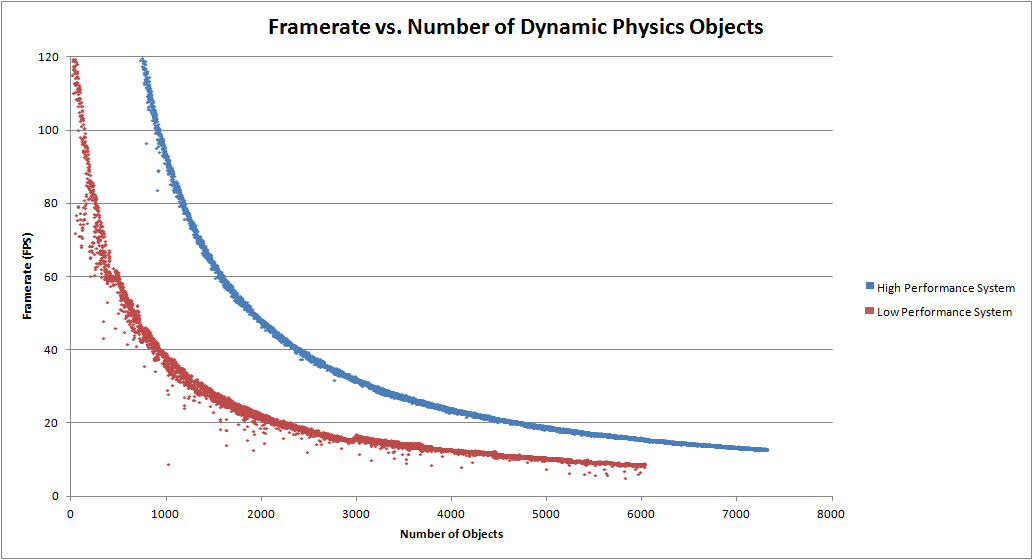
\includegraphics[width=\textwidth]{frameratedynamic}
\caption{Framerate vs. number of dynamic objects} \label{fig:frdynamic}
\end{figure}

\begin{figure}[htb]
\centering
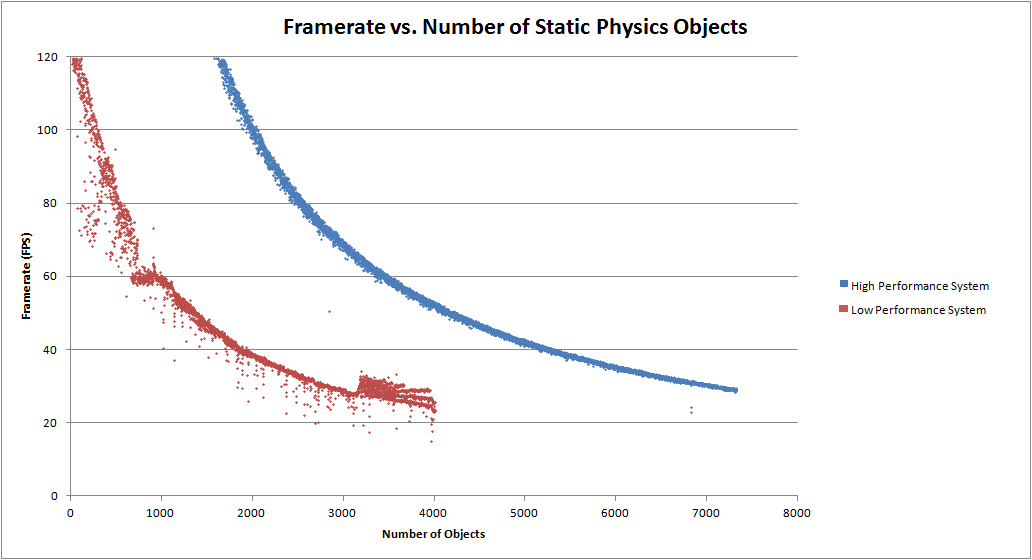
\includegraphics[width=\textwidth]{frameratestatic}
\caption{Framerate vs. number of static objects} \label{fig:frstat}
\end{figure}

\FloatBarrier

A plot showing the variation in framerate with respect to the number of platforms was also produced and is shown in \hyperref[fig:frplat]{Figure~\ref*{fig:frplat}}.  The results of this test show a drastic drop in framerate with very few objects, and this framerate drop appears to be consistent between the high end and low end systems.  This suggests that the problem is in using multiple shaders:  switching shaders is a resource intensive procedure and the consistencies in framerate between the two systems can be explained by the fact that the amount of time required for switching a shader would be approximately constant between the two systems.  This problem was fixed by combining the three platform shaders into one shader.  This change required only minor minor changes to the rendering code.




\begin{figure}[htb]
\centering
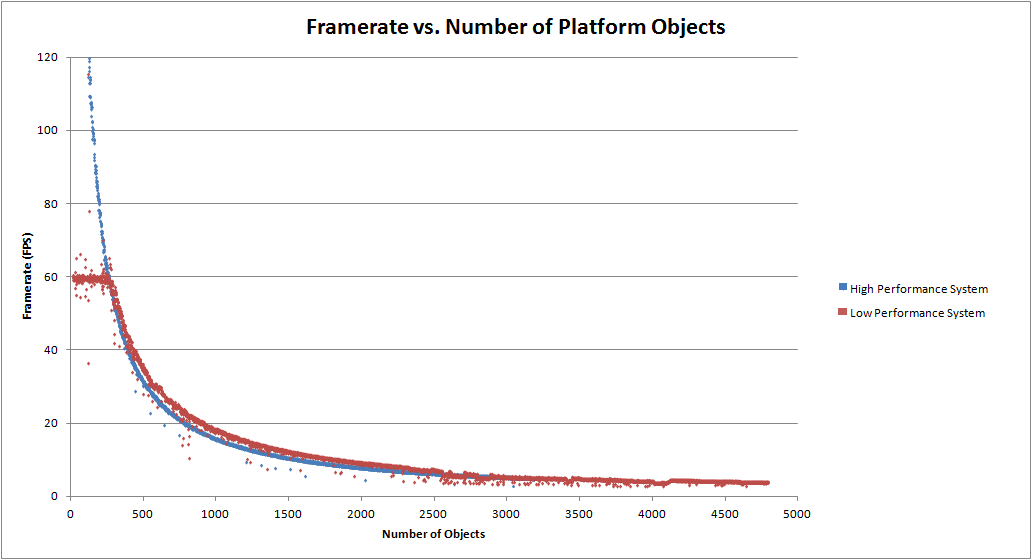
\includegraphics[width=\textwidth]{framerateplat}
\caption{Framerate vs. number of platform objects} \label{fig:frplat}
\end{figure}
\FloatBarrier


Additional testing was performed to assess whether the framerate was predominantly affected by procedures involving physics calculations or rendering.  The results of these tests are given in \hyperref[fig:isohi]{Figure~\ref*{fig:isohi}} and \hyperref[fig:isolo]{Figure~\ref*{fig:isolo}} for the high and low performance systems, respectively.  Interestingly, from the plot of the high performance system it appears that neither is a dominant factor:  both make a roughly equal contribution to the overall framerate.  This does not appear to be the case in the low performance system, where it is clear that the rendering step limits the framerate.

\begin{figure}[htb]
\centering
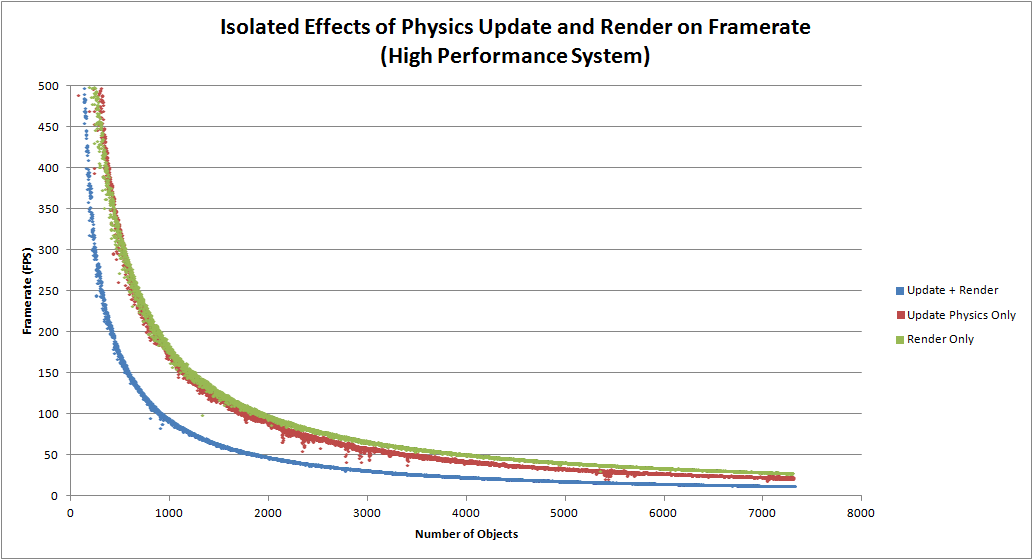
\includegraphics[width=\textwidth]{isolatedhigh}
\caption{Effects of physics update and render on framerate on high performance system} \label{fig:isohi}
\end{figure}


\begin{figure}[htb]
\centering
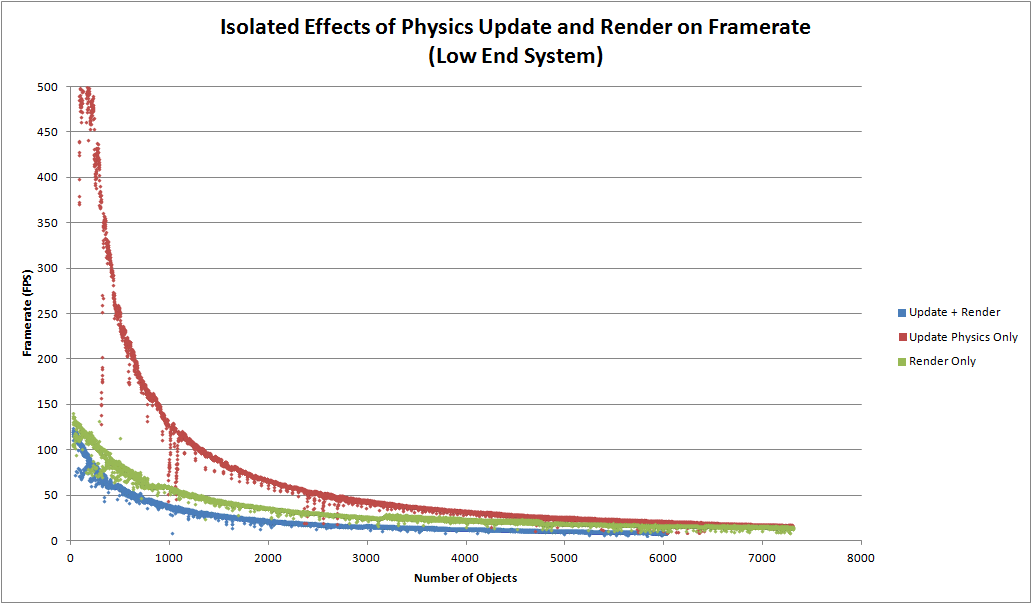
\includegraphics[width=\textwidth]{isolatedlo}
\caption{Effects of physics update and render on framerate on low performance system} \label{fig:isolo}
\end{figure}

\FloatBarrier

\testmanual{
    name = Hardware requirements,
    desc = Tests for the minimum hardware requirements required to maintain an average frame rate of at least $\hyperref[tab:constants]{\sigma}$ frames per second,
    type = {Functional (dynamic, manual)},
    user = {Development team},
    pass = Game maintains frame rate of at least $\hyperref[tab:constants]{\sigma}$ frames per second in a stage that contains $\hyperref[tab:constants]{\Phi}$ dynamic objects when tested on a low-performance system,
    result = \textcolor{Orange}{Borderline PASS due to platform shader performance}
}

\section{Future Testing}
\subsection{Usability Testing}
A user experience survey will be carried out to assess useability.  This survey will be administered in the future (date to be determined) and the results will therefore not be a part of the project submission.  

\testmanual{
    name = {Entertainment},
    desc = Tests that the game is entertaining,
    type = {Functional (dynamic, manual)},
    user = {Testing group},
    pass = {Average survey score of at least $\hyperref[tab:constants]{\Theta}$},
    result = \textcolor{Orange}{Planned for future (TBD)}
}

\testmanual{
    name = {Challenge},
    desc = Tests that the game is adequately challenging (not too easy or too hard),
    type = {Functional (dynamic, manual)},
    user = {Testing group},
    pass = {Average survey score within $\hyperref[tab:constants]{\Psi}$ of 5}
    result = \textcolor{Orange}{Planned for future (TBD)}
}

\testmanual{
    name = {Controls},
    desc = Tests that the game controls are intuitive,
    type = {Functional (dynamic, manual)},
    user = {Testing group},
    pass = {Average survey score of at least $\hyperref[tab:constants]{\Omega}$}
    result = \textcolor{Orange}{Planned for future (TBD)}
}

\subsection{Robustness Testing}
Robustness of the application with regard to erroneous input was not formally tested.  User inputs are only accepted as defined keystrokes and mouse clicks.  The way these inputs map to setting/modifying variables is entirely controlled by the game code and thus the user is never able to directly change any variables via inputs.  This means that all variables are maintained within their expected ranges and no explicit testing is required.

Robustness tests in the form of stress testing were covered under performance testing.

\section{Summary of Changes}
A summary of the changes made in response to testing are given in \hyperref[tab:changes]{Table~\ref*{tab:changes}}.  Few changes were made to the game as a result of the tests described in this document.  This is due to the fact that informal testing was performed constantly as the game was being developed.  Every time changes were made to the game code or new features were added, the game was compiled and played by the development team to ensure that everything was working as intended.  Anything that did not work properly was fixed on the spot.

\begin{table}[ht]
\caption{Changes made in response to testing} \label{tab:changes}
\begin{tabularx}{\textwidth}{p{5cm}X}
\toprule {\bf Test} & {\bf Changes Made}\\
\midrule
28 & Surface objects were originally rendered using three separate shaders to handle texture wrapping in different planes.  The shaders were combined into one shader that uses different pathways depending on a variable passed in by the game.  This required only minor modifications to the Obj class render function.\\
\bottomrule
\end{tabularx}
\end{table}

\section{Traceability}
\subsection{Trace of Testing to Requirements}
A trace between requirements and testing is given in \hyperref[tab:tracereq]{Table~\ref*{tab:tracereq}}.\\

\begin{table}[h]
\caption{Trace between requirements and tests} \label{tab:tracereq}
\centering
\begin{tabularx}{0.55\textwidth}{p{4cm}X}
\toprule {\bf Requirement} & {\bf Test(s)}\\
\midrule
1	&	24	\\
2	&	24	\\
3	&	24	\\
4	&	24	\\
5	&	2, 4	\\
6	&	3, 5	\\
7	&	6	\\
8	&	11	\\
9	&	16\\
10	&	19	\\
11	&	18	\\
12	&	12	\\
13	&	13	\\
14	&	9, 10	\\
15	&	7, 8	\\
16	&	14, 17	\\
17	&	14	\\
18	&	15	\\
19	&	24	\\
20	&	25	\\
21	&	25	\\
22	&	20, 21, 25	\\
23	&	22, 23	\\
24	&	29	\\
25	&	31	\\
26	&	30	\\
27	&	28	\\
28  &    26   \\
29  &    27   \\
\bottomrule
\end{tabularx}
\end{table}
\subsection{Trace of Testing to Modules}
A trace between modules and testing is given in \hyperref[tab:tracemod]{Table~\ref*{tab:tracemod}}.\\

\begin{table}[ht]
\caption{Trace between modules and tests} \label{tab:tracemod}
\centering
\begin{tabularx}{0.55\textwidth}{p{5cm}X}
\toprule {\bf Module} & {\bf Test(s)}\\
\midrule
1	&	28	\\
2	&	20, 21	\\
3	&	20, 21	\\
4	&	20, 21	\\
5	&	16, 17	\\
6	&	17	\\
7	&	17	\\
8	&	9, 10, 17	\\
9	&	7, 8, 17\\
10	&	17	\\
11	&	15	\\
12	&	16, 17	\\
13	&	14, 16, 17	\\
14	&	14, 16, 17	\\
15	&	16, 17	\\
16	&	16, 17	\\
17	&	2-17	\\
18	&	16, 17	\\
19	&	20, 21	\\
20	&	20, 21	\\
21	&	20, 21	\\
22	&	2-15, 24	\\
23	&	24	\\
24	&	2-15	\\
25	&	24	\\
26	&	12, 13	\\
27	&	22, 23	\\
28  &    22, 23   \\
29  &    20, 21   \\
30 & 20, 21\\
\bottomrule
\end{tabularx}
\end{table}



\end{document}
